%插入样式内容
\documentclass[12pt]{article}
%%---------------------------------------------------------------------
% packages
% geometry
\usepackage{geometry}
% font
\usepackage{fontspec}
\defaultfontfeatures{Mapping=tex-text}  %%如果没有它,会有一些 tex 特殊字符无法正常使用,比如连字符。
\usepackage{xunicode,xltxtra}
\usepackage[BoldFont,SlantFont,CJKnumber,CJKchecksingle]{xeCJK}  % \CJKnumber{12345}: 一万二千三百四十五
\usepackage{CJKfntef}  %%实现对汉字加点、下划线等。
\usepackage{pifont}  % \ding{}
% math
\usepackage{amsmath,amsfonts,amssymb}
% color
\usepackage{color}
\usepackage{xcolor}
\definecolor{EYE}{RGB}{199,237,204}
\definecolor{FLY}{RGB}{128,0,128}
\definecolor{ZHY}{RGB}{139,0,255}
% graphics
\usepackage[americaninductors,europeanresistors]{circuitikz}
\usepackage{tikz}
\usetikzlibrary{positioning,arrows,shadows,shapes,calc,mindmap,trees,backgrounds}  % placements=positioning
\usepackage{graphicx}  % \includegraphics[]{}
\usepackage{subfigure}  %%图形或表格并排排列
% table
\usepackage{colortbl,dcolumn}  %% 彩色表格
\usepackage{multirow}
\usepackage{multicol}
\usepackage{booktabs}
% code
\usepackage{fancyvrb}
\usepackage{listings}
% title
\usepackage{titlesec}
% head/foot
\usepackage{fancyhdr}
% ref
\usepackage{hyperref}
% pagecolor
\usepackage[pagecolor={EYE}]{pagecolor}
% tightly-packed lists
\usepackage{mdwlist}

\usepackage{styles/iplouccfg}
\usepackage{styles/zhfontcfg}
\usepackage{styles/iplouclistings}

\usepackage{color,framed}

%%---------------------------------------------------------------------
% settings
% geometry
\geometry{left=2cm,right=1cm,top=2cm,bottom=2cm}  %设置 上、左、下、右 页边距
\linespread{1.5} %行间距
% font
\setCJKmainfont{Adobe Kaiti Std}
%\setmainfont[BoldFont=Adobe Garamond Pro Bold]{Apple Garamond}  % 英文字体
%\setmainfont[BoldFont=Adobe Garamond Pro Bold,SmallCapsFont=Apple Garamond,SmallCapsFeatures={Scale=0.7}]{Apple Garamond}  %%苹果字体没有SmallCaps
\setCJKmonofont{Adobe Fangsong Std}
% graphics
\graphicspath{{figures/}}
\tikzset{
    % Define standard arrow tip
    >=stealth',
    % Define style for boxes
    punkt/.style={
           rectangle,
           rounded corners,
           draw=black, very thick,
           text width=6.5em,
           minimum height=2em,
           text centered},
    % Define arrow style
    pil/.style={
           ->,
           thick,
           shorten <=2pt,
           shorten >=2pt,},
    % Define style for FlyZhyBall
    FlyZhyBall/.style={
      circle,
      minimum size=6mm,
      inner sep=0.5pt,
      ball color=red!50!blue,
      text=white,},
    % Define style for FlyZhyRectangle
    FlyZhyRectangle/.style={
      rectangle,
      rounded corners,
      minimum size=6mm,
      ball color=red!50!blue,
      text=white,},
    % Define style for zhyfly
    zhyfly/.style={
      rectangle,
      rounded corners,
      minimum size=6mm,
      ball color=red!25!blue,
      text=white,},
    % Define style for new rectangle
    nrectangle/.style={
      rectangle,
      draw=#1!50,
      fill=#1!20,
      minimum size=5mm,
      inner sep=0.1pt,}
}
\ctikzset{
  bipoles/length=.8cm
}
% code
\lstnewenvironment{VHDLcode}[1][]{%
  \lstset{
    basicstyle=\footnotesize\ttfamily\color{black},%
    columns=flexible,%
    framexleftmargin=.7mm,frame=shadowbox,%
    rulesepcolor=\color{blue},%
%    frame=single,%
    backgroundcolor=\color{yellow!20},%
    xleftmargin=1.2\fboxsep,%
    xrightmargin=.7\fboxsep,%
    numbers=left,numberstyle=\tiny\color{blue},%
    numberblanklines=false,numbersep=7pt,%
    language=VHDL%
    }\lstset{#1}}{}
\lstnewenvironment{VHDLmiddle}[1][]{%
  \lstset{
    basicstyle=\scriptsize\ttfamily\color{black},%
    columns=flexible,%
    framexleftmargin=.7mm,frame=shadowbox,%
    rulesepcolor=\color{blue},%
%    frame=single,%
    backgroundcolor=\color{yellow!20},%
    xleftmargin=1.2\fboxsep,%
    xrightmargin=.7\fboxsep,%
    numbers=left,numberstyle=\tiny\color{blue},%
    numberblanklines=false,numbersep=7pt,%
    language=VHDL%
    }\lstset{#1}}{}
\lstnewenvironment{VHDLsmall}[1][]{%
  \lstset{
    basicstyle=\tiny\ttfamily\color{black},%
    columns=flexible,%
    framexleftmargin=.7mm,frame=shadowbox,%
    rulesepcolor=\color{blue},%
%    frame=single,%
    backgroundcolor=\color{yellow!20},%
    xleftmargin=1.2\fboxsep,%
    xrightmargin=.7\fboxsep,%
    numbers=left,numberstyle=\tiny\color{blue},%
    numberblanklines=false,numbersep=7pt,%
    language=VHDL%
    }\lstset{#1}}{}
% pdf
\hypersetup{%pdfpagemode=FullScreen,%
            pdfauthor={Haiyong Zheng},%
            pdftitle={Title},%
            CJKbookmarks=true,%
            bookmarksnumbered=true,%
            bookmarksopen=false,%
            plainpages=false,%
            colorlinks=true,%
            citecolor=green,%
            filecolor=magenta,%
            linkcolor=cyan,%red(default)
            urlcolor=cyan}
% section
%http://tex.stackexchange.com/questions/34288/how-to-place-a-shaded-box-around-a-section-label-and-name
\newcommand\titlebar{%
\tikz[baseline,trim left=3.1cm,trim right=3cm] {
    \fill [cyan!25] (2.5cm,-1ex) rectangle (\textwidth+3.1cm,2.5ex);
    \node [
        fill=cyan!60!white,
        anchor= base east,
        rounded rectangle,
        minimum height=3.5ex] at (3cm,0) {
        \textbf{\thesection.}
    };
}%
}
\titleformat{\section}{\Large\bf\color{blue}}{\titlebar}{0.1cm}{}
% head/foot
\setlength{\headheight}{15pt}
\pagestyle{fancy}
\fancyhf{}

\chead{\color{black!50!green}DIGITS DevBox}

%\lfoot{\color{blue!50!green}Dai Jialun}
\cfoot{\color{blue!50!green}\href{http://vision.ouc.edu.cn/~zhenghaiyong}{CVBIOUC}}
\rfoot{\color{blue!50!green}$\cdot$\ \thepage\ $\cdot$}
\renewcommand{\headrulewidth}{0.4pt}
\renewcommand{\footrulewidth}{0.4pt}


%%---------------------------------------------------------------------
\begin{document}
%%---------------------------------------------------------------------
%%---------------------------------------------------------------------
% \titlepage
\title{\vspace{-2em} DIGITS DevBox深度学习服务器\\
\normalsize{}}
\author{Dai Jialun}
\date{\vspace{-0.7em} \today \vspace{-0.7em}}
%%---------------------------------------------------------------------
\maketitle\thispagestyle{fancy}
%%---------------------------------------------------------------------
\maketitle
%\tableofcontents 
\section{硬件配置}
\begin{description}
\item[显卡] 4个ASUS(华硕)GTX 980Ti-6GD5
\definecolor{shadecolor}{rgb}{0.92,0.92,0.92}  
\begin{shaded}
\scriptsize{
芯片厂商: NVIDIA

显卡芯片: GeForce GTX 980Ti

显示芯片系列: NVIDIA GTX 900系列

核心代号: GM200

显存类型: GDDR5

显存容量: 6144MB

显存位宽: 384bit

最大分辨率: 4096×2160

接口类型: PCI Express 3.0 16X

I/O接口: HDMI接口/DVI接口/3个DisplayPort接口

电源接口: 8pin+6pin

产品尺寸:266.7×111.2×38.1mm

参考报价:5999*4=23996} 
\end{shaded}   
\item[CPU] 1个Intel(英特尔) Core i7-5960X
\definecolor{shadecolor}{rgb}{0.92,0.92,0.92}  
\begin{shaded}
\scriptsize{
CPU主频:3GHz

最高睿频:3.5GHz 

总线类型:QPI总线

总线频率:8GT/s

插槽:LGA 2011-v3 

CPU架构:Haswell

核心:八核心十六线程

制作工艺: 22纳米

功耗: 140W

三级缓存: 20MB

最大支持内存:64G

指令集:SSE4.2,AVX 2.0,AES

内存控制器:四通道:DDR4 1333/1600/2133

参考报价: 7699 RMB} 
\end{shaded}   
\item[主板] 1个ASUS(华硕)X99-E WS
\definecolor{shadecolor}{rgb}{0.92,0.92,0.92}  
\begin{shaded}
\scriptsize{
主芯片组:Intel X99

CPU插槽:LGA 2011-3

支持CPU数量: 1颗

内存类型: DDR4

内存插槽: 8*DDR4 DIMM

最大内存容量: 128GB

内存描述:支持四通道DDR4 3000(超频)/3200(O.C.)/2800(超频)/2666(超频)/2400(超频)/2133MHz内存

显卡插槽: PCI-E 3.0标准

PCI-E插槽:7×PCI-E X16显卡插槽

SATA接口: 8×SATA III接口;1×SATA Express接口;1×M.2接口(10Gb/s)

USB接口: 12×USB3.0接口(10背板+2内置);4×USB2.0接口(2背板+2内置)

版型:E-ATX板型

外形尺寸:30.5×26.7cm 

多显卡技术:支持NVIDIA 4-Way SLI四路交火技术

RAID功能:支持RAID 0,1,5,10 

尺寸:30.5 厘米 x 26.7 厘米

参考报价: 4799 RMB} 
\end{shaded}   
\item[内存] 2个CORSAIR(海盗船) VENGERNCE(复仇者)LPX 32GB(4 $\times$ 8GB) DDR4 2400MHz CMK32GX4M4A2400C14R
\definecolor{shadecolor}{rgb}{0.92,0.92,0.92}  
\begin{shaded}
\scriptsize{
内存容量:套装(4×8GB)

内存类型:DDR4

内存主频:2400MHz

参考报价:5000*2=10000 RMB} 
\end{shaded} 
\item[硬盘] 3个WesternDigital(西部数码) 4TB 7200转
\definecolor{shadecolor}{rgb}{0.92,0.92,0.92}  
\begin{shaded}
\scriptsize{
硬盘容量:4000G

缓存:64M

转速:7200rpm

接口类型:SATA3.0

接口速率:6Gb/s

参考报机:1799*3=5397 RMB} 
\end{shaded} 
\item[固态硬盘] 1个Samsung(三星)SSD 850pro 512GB
\definecolor{shadecolor}{rgb}{0.92,0.92,0.92}  
\begin{shaded}
\scriptsize{
接口类型:SATA3

硬盘尺寸:2.5英寸

参考报价:2999 RMB} 
\end{shaded} 
\item[固态硬盘] 1个Samsung SSD 512GB SM951 cache for RAID
\definecolor{shadecolor}{rgb}{0.92,0.92,0.92}  
\begin{shaded}
\scriptsize{
参考报价:3450 RMB} 
\end{shaded} 
\item[机箱] 1个CORSAIR(海盗船) 900D
\begin{shaded}
\scriptsize{
机箱样式:台式机箱(全塔)

适用主板:**EATX板型**,ATX板型,MATX板型

电源类型:标准ATX PS2电源(选配)

电源设计:下置电源

显卡限长:400mm

5.25英寸仓位:4个

3.5英寸仓位:9个

2.5英寸仓位:9个

扩展插槽:10

前置接口:4*USB 2.0;2*USB 3.0

散热性能:前:3×120mm风扇(标配),
   	顶:4×120mm或3*140mm风扇(选配),
        后:1×140mm风扇(标配),
        底:8×120mm或6*140mm风扇(选配)

尺寸:649.6×252×691.6mm

参考报价:2499 RMB } 
\end{shaded} 
\item[电源] 1个CORSAIR(海盗船) AX1500i 1500W
\definecolor{shadecolor}{rgb}{0.92,0.92,0.92}  
\begin{shaded}
\scriptsize{
功率:1500W

风扇描述:14cm风扇

电源尺寸:150x86x225mm

参考报价:3599 RMB} 
\end{shaded} 
\item[散热器] 1个CORSAIR(海盗船) H110 水冷CPU散热器
\definecolor{shadecolor}{rgb}{0.92,0.92,0.92} 
\begin{shaded}
\scriptsize{
参考报价:999 RMB} 
\end{shaded} 
\item[风扇] 6个CORSAIR(海盗船)AF120 静音版 双包装
\definecolor{shadecolor}{rgb}{0.92,0.92,0.92} 
\begin{shaded}
\scriptsize{
参考报价:89*12=1068 RMB} 
\end{shaded} 
\item[光驱] 1个AUSU(华硕)DRW-24D1ST
\definecolor{shadecolor}{rgb}{0.92,0.92,0.92} 
\begin{shaded}
\scriptsize{
参考报价:120 RMB} 
\end{shaded} 
\item[配件] 1个Thermaltake Commander FT触控式面板风扇控制器,Deepcool FAN HUB(九州风神风扇集线器)
\definecolor{shadecolor}{rgb}{0.92,0.92,0.92} 
\begin{shaded}
\scriptsize{
参考报价:299 RMB} 
\end{shaded} 
\item[显示器]
\item[键盘鼠标]
\end{description}

\section{名词解释}
\begin{description}

\item[DVI] Digital Visual Interface,数字视频接口
\begin{figure}[!h]
\centering
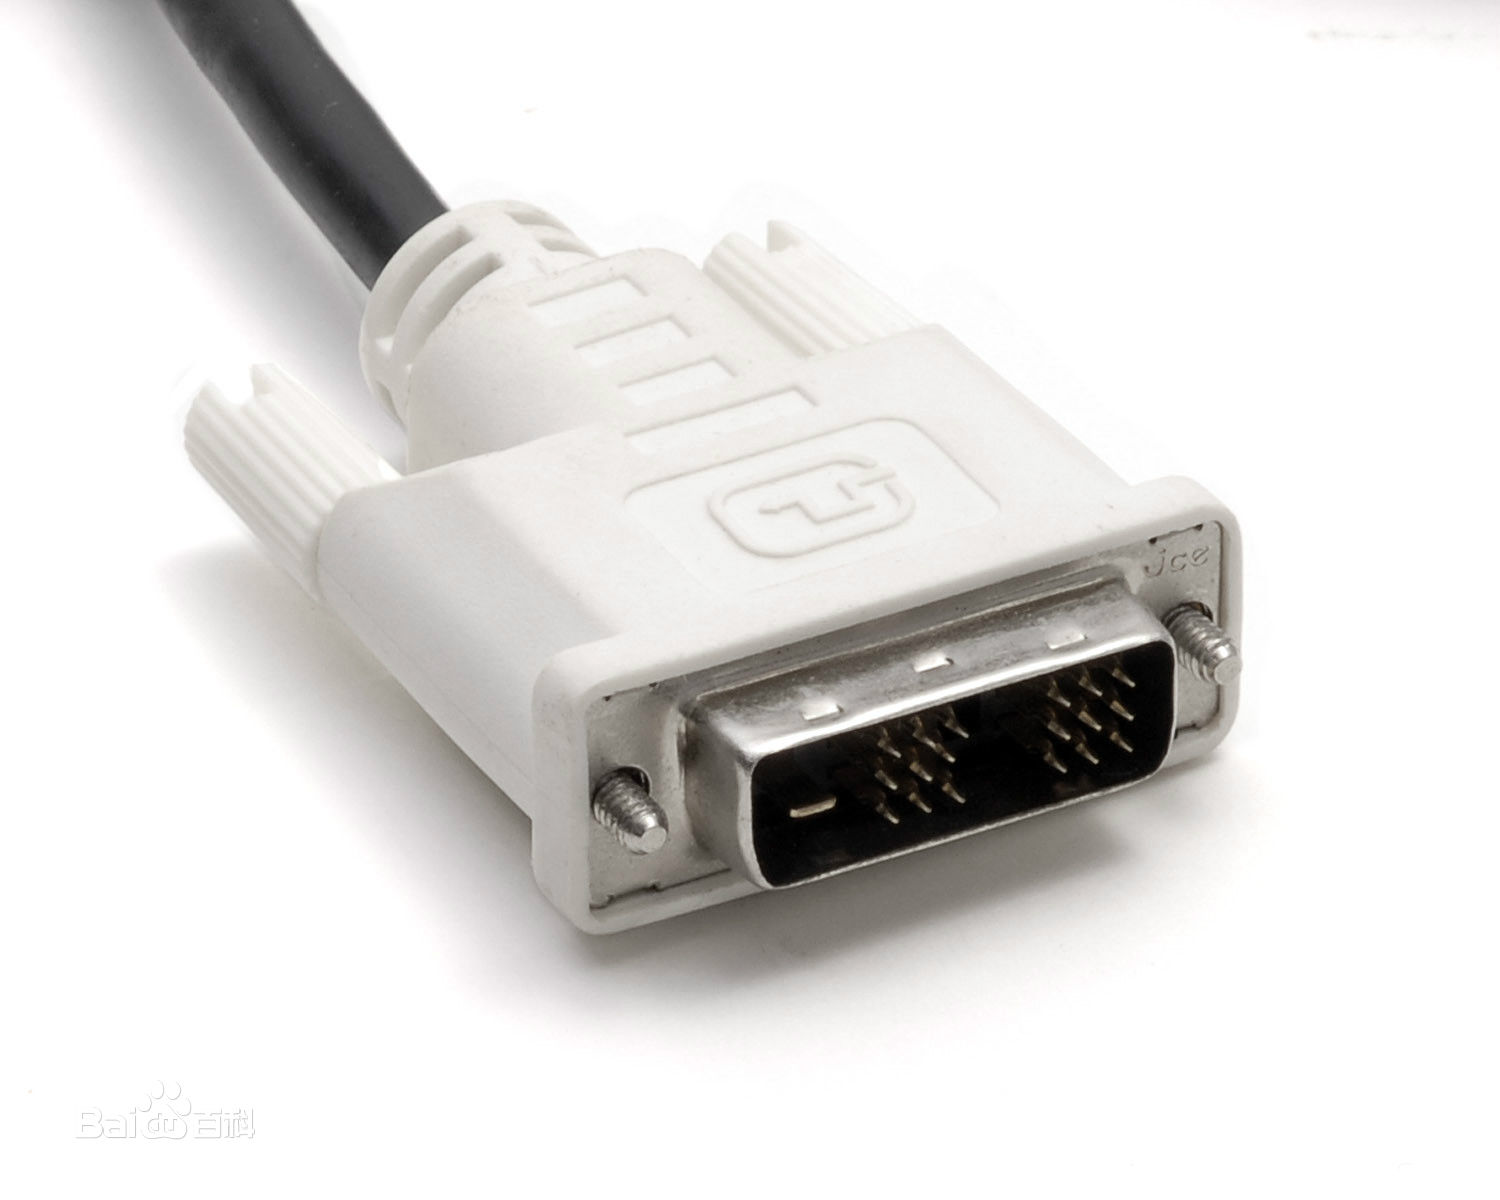
\includegraphics[width=0.2\textwidth]{DVI}
\end{figure}

\item[DislayPort] 高清数字显示借口标准
\begin{figure}[!ht]
\centering
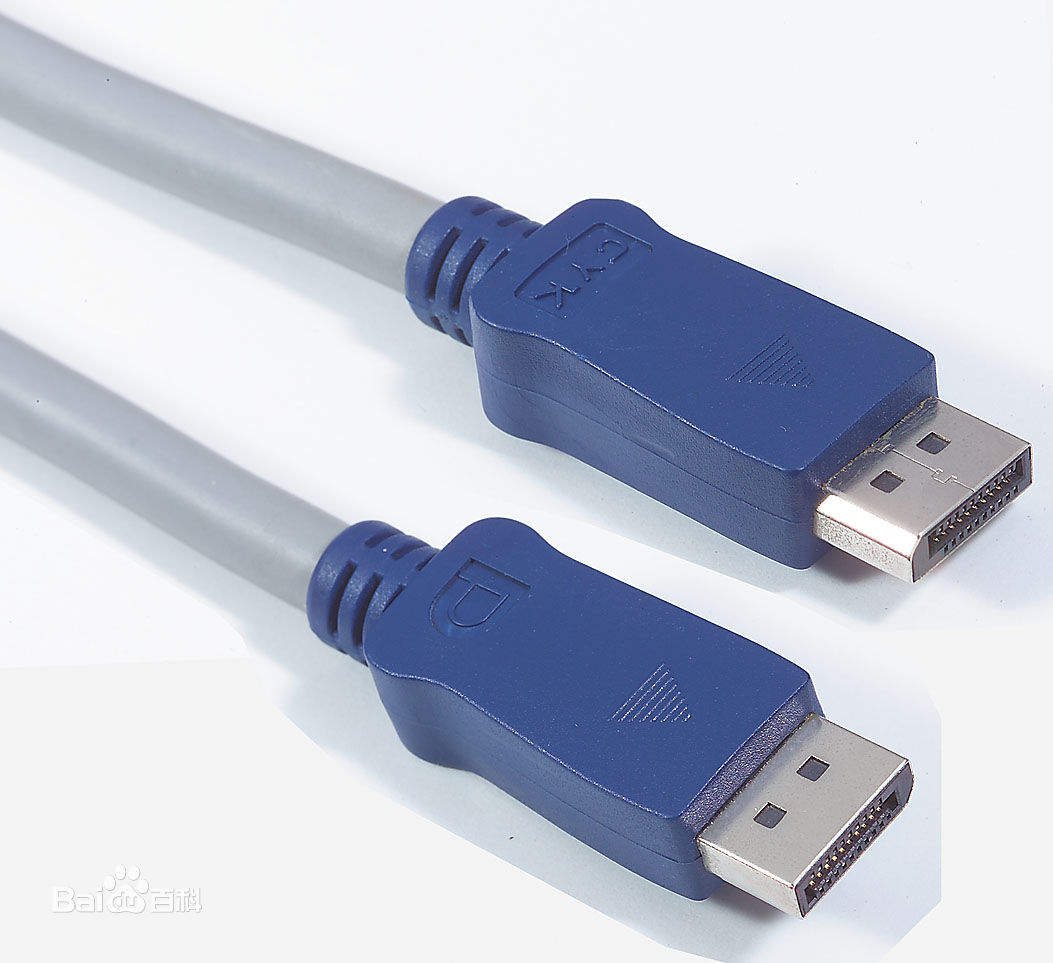
\includegraphics[width=0.2\textwidth]{DisplayPort}
\end{figure}

\item[PCI-E] PCI Express,新的总线接口
\begin{figure}[!ht]
\centering
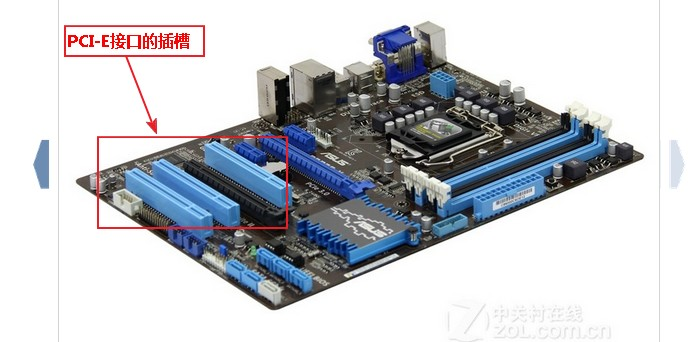
\includegraphics[width=0.2\textwidth]{PCI-E}
\end{figure}

\item[SATA Revision 3.0] Serial Advanced Technology Attachment,串行ATA规格第三版,6Gbps
\begin{figure}[!ht]
\centering
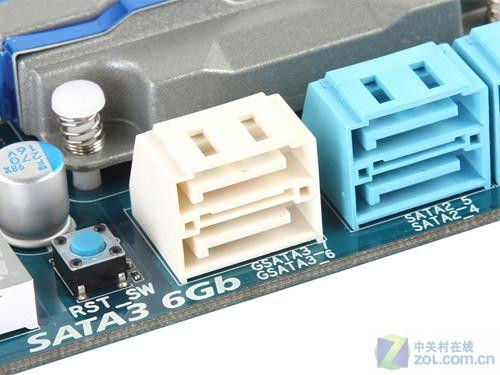
\includegraphics[width=0.2\textwidth]{SATA3}
\end{figure}

\item[SATA EXpress] SATA 3.0下一代的SATA接口,10Gbps
\begin{figure}[!ht]
\centering
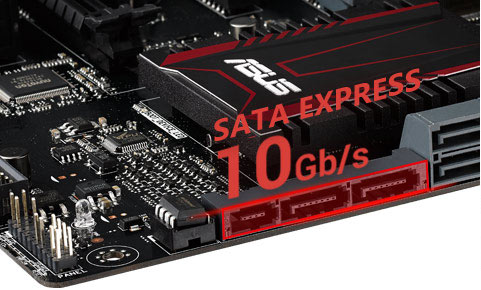
\includegraphics[width=0.2\textwidth]{SATAE}
\end{figure}

\item[M.2] 一种替代MSATA新的接口规范,优势体现在速度和体积。支持Socket2和Socket3两种接口类型
\begin{figure}[!ht]
  \centering 
  \subfigure[]{ 
    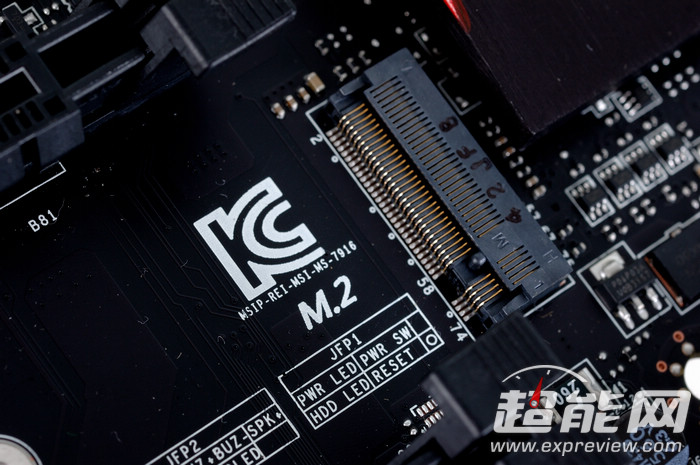
\includegraphics[width=0.23\textwidth]{M2}} 
  \subfigure[]{ 
    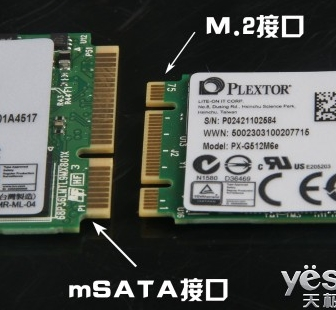
\includegraphics[width=0.17\textwidth]{M2-MSATA}} 
  \caption{}
\end{figure}

\item[RAID] Redundant Arrays of Independent Disks,磁盘阵列。磁盘阵列是由很多价格较便宜的磁盘,组合成一个容量巨大的磁盘组,利用个别磁盘提供数据所产生加成效果提升整个磁盘系统效能。利用这项技术,将数据切割成许多区段,分别存放在各个硬盘上。
\begin{figure}[!ht]
  \centering 
  \subfigure[]{ 
    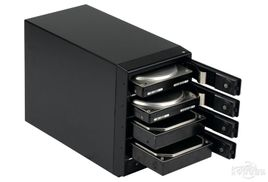
\includegraphics[width=0.24\textwidth]{RAID1}} 
  \subfigure[]{ 
    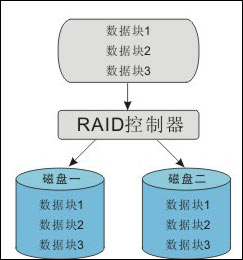
\includegraphics[width=0.15\textwidth]{RAID2}} 
  \caption{}
\end{figure}

\item[RAID5] 一种存储性能、数据安全和存储成本兼顾的存储解决方案。为系统提供数据安全保障,但保障程度要比Mirror低而磁盘空间利用率要比Mirror高。数据以块为单位分布到各个硬盘上。RAID 5不对数据进行备份,而是把数据和与其相对应的奇偶校验信息存储到组成RAID5的各个磁盘上,并且奇偶校验信息和相对应的数据分别存储于不同的磁盘上。当RAID5的一个磁盘数据损坏后,利用剩下的数据和相应的奇偶校验信息去恢复被损坏的数据。
\begin{figure}[!ht]
\centering
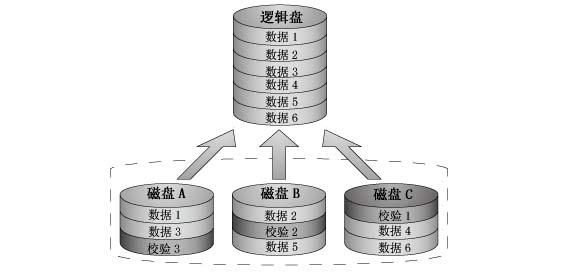
\includegraphics[width=0.4\textwidth]{RAID5}
\end{figure}

\item[SLI] Scalable Link Interface,可灵活伸缩的连接接口(支持多显卡技术)。这是一种可把两张或以上的显卡连在一起,作单一输出使用的技术,从而达至绘图处理效能加强的效果。
\begin{figure}[!ht]
\centering
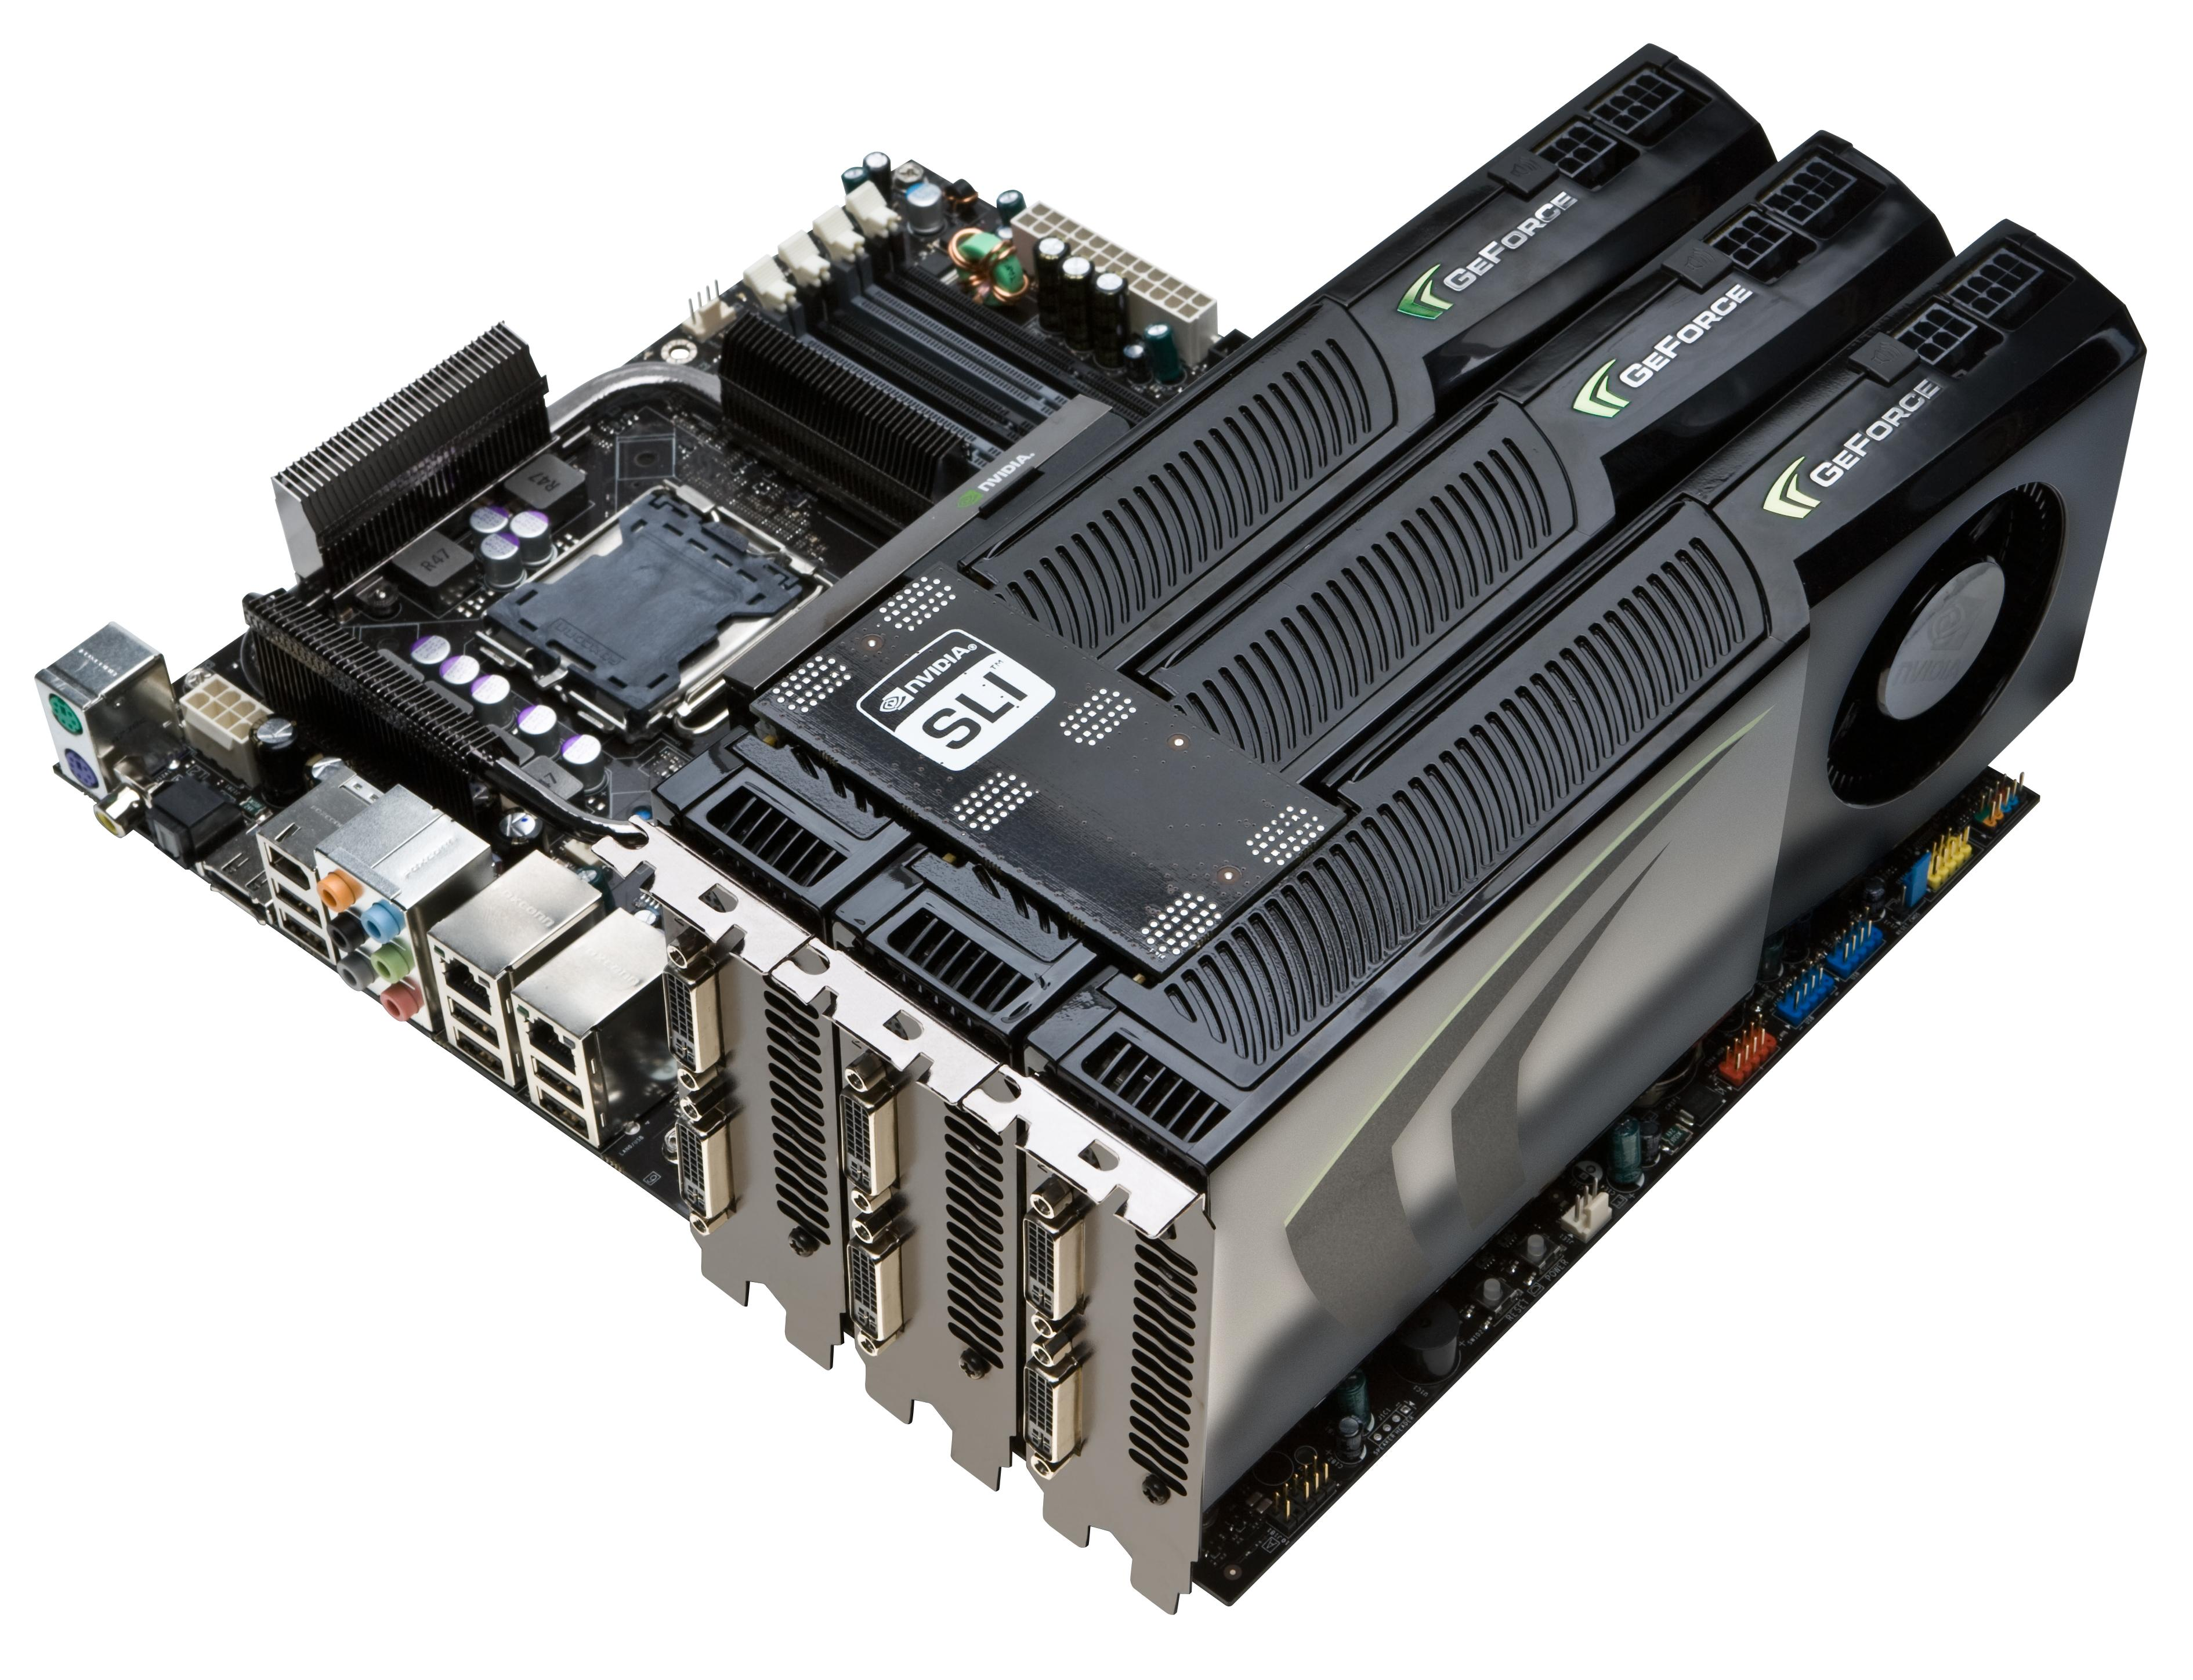
\includegraphics[width=0.2\textwidth]{SLI}
\end{figure}

\item[DDR4] Dual Data Rate SDRAM,是一种高速CMOS动态随即访问的内存。DDR4支持2133MHz,32GB DDR4-2133达到48.4GB/s。

\item[GDDR5] Graphics Double Data Rate SDRAM version5,是一种高性能显卡用内存,需搭配支持PCI-E以上规格的显卡,高频率达4GHZ,低功耗。
\end{description}

\section{软件配置名词}
\begin{description}
\item[UEFI] Unified Extensible Firmware Interface,统一的可扩展固件接口,是一种详细描述类型接口的标准。这种接口用于操作系统自动从预启动的操作环境,加载到一种操作系统上。
\item[BIOS] Basic Input/Output System,基本输入/输出系统。
\item[固件] Firmware,固定软件(自己理解),写入EROM或EEPROM中的程序。固件担任着一个系统最基础最底层工作的软件。初期,这些硬件内所保存的程序是无法被用户直接读出或修改的,如今这些是可以重复刷写的,让固件得以修改和升级。
\end{description}

\section{环境配置}


\subsection{创建RAID5}
\subsubsection{RAID的优点}
\begin{itemize}
\item 可高效恢复磁盘
\item 增强了速度
\item 扩容了存储能力
\end{itemize}

\subsubsection{RAID的分类}
\begin{description}
\item[硬RAID] Hardware RAID,通过用硬件(RAID卡或者磁盘阵列)来实现RAID功能。硬件RAID具备了自身的RAID控制/处理与I/O处理芯片,甚至还有阵列缓冲(Array Buffer),对CPU的占用率以及整体性能都是最优势的,但设备成本也是三最高的。Hardware RAID自成一个单元,由自身硬件和软件管理RAID,与主板和操作系统无关,即Ubuntu不需要额外的程序来管理。
\item[软RAID] Software RAID,通过用操作系统的软件程序(Linux系统下的mdadm命令)来完成RAID功能。软件RAID的所有功能都是操作系统与CPU 来完成,没有第三方的控制/处理与I/O 芯片,与主板BIOS程序无关,其效率与稳定性较低。例如在Ubuntu系统下的软RAID,其格式化、挂载、写入与重建全部由mdadm负责。
\item[伪RAID] Fake RAID,又称BIOS RAID。通过主板的集成芯片,内建RAID控制器来创建阵列,由操作系统驱动识别(主要表现在Intel Desktop的主板上表现的比较明显)。由于缺乏独立的I/O处理芯片,所以这方面的工作仍要由CPU与驱动程序来完成。另外,Fake RAID所采用的RAID控制/处理芯片的能力一般都比较弱,不能支持高的RAID等级。在Intel集成芯片的主板,主要使用Intel Rapid Storage Technology来管理,该技术主要支持Window系统,不支持Linux系统。在Linux系统下,Intel主要使用dmraid和mdadm来管理RAID,推荐使用mdadm。
\end{description}

\subsubsection{主板集成RAID与外插RAID卡区别}
\begin{description}
\item[性能] 主板集成的RAID,它的性能以及速度是通过主板的CPU与内存来实现的,它会占有主板一定的带宽,会影响整机的性能;外插RAID卡,有自己的CPU和内存,所以数据处理大部分都会独立处理,不会影响主板上的CPU与内存速度。总体看来,外插的RAID卡的RAID要比主板集成的RAID快得多。
\item[安全性] 主板集成的RAID,其安全性不能够得到保证,因为是通过更改主板的BIOS选项做成的,所以一旦主板损坏、主板的CMOS电池掉电或无意更改了主板BIOS的设置都会带来RAID的丢失。通过主板做成的RAID,一旦丢失,将会不能恢复,后果是非常严重的;而外插的RAID卡所做成的RAID,不会因为主板损坏、主板的CMOS电池掉电等现象对数据造成影响,所以外插的RAID卡,其安全性远远大于主板集成的。另外,Raid完全由Ubuntu的mdadm命令管理。
\end{description}


\subsubsection{创建RAID5步骤(Fake RAID,在BISO界面)}
\begin{enumerate}
\item 初始化,对各个磁盘删除分区(fdisk命令),且进行格式化(mkfs命令)。小容量硬盘(不到2TB)使用MRB分区表,大容量硬盘(2TB以上)使用GPT分区,\footnote{http://wangheng.org/shi-yong-parted-chuang-jian-gpt-fen-qu.html}。
\begin{bash}
sudo fdisk -l		   #查看磁盘空间以及分区
sudo fdisk /dev/sdX  #用fdisk对某块硬盘处理,/dev/sdX中X表示磁盘号,例如/dev/sdb
sudo mkfs.ext4 /dev/sdX    #用mkfs将/dev/sdX格式化为ext4格式
sudo parted /dev/sdX	#用parted工具对大容量硬盘分区,为GPT分区
\end{bash}
MRB分区表是将磁盘的分区信息保存到磁盘的第一个扇区
\item 创建,create
\item 分配,
\item 格式化 sudo mkfs.ext4 /dev/sdb
\item 挂载 sudo /dev/mapper/isw\_dfafd\_Volume1 /deep
\item 自动挂载 sudo vim /etc/fstab
\end{enumerate}

可能出现问题
\begin{itemize}
\item 在装系统过程中,在选择系统分区时,ctrl+alt+F1,输入dmraid -ay激活RAID(Ubuntu server) 这种方式其实还是属于介于软raid与硬raid之间。在启动时候,由硬件raid驱动,当载入linux内核之后,由linux接手管理,还是会消耗cpu等资源。与更传统的软件raid比较,就是启动的时候(linux内核未介入之前)系统看到的仍然是一个raid的虚拟硬盘,所以两快硬盘完全一样,要恢复重建之类的更加简单。另外的话,dmraid映射了底层的硬件raid驱硬件控制器,raid控制可能也能帮助处理一些操作,可能对性能也会有一定提高。 
\item dmraid将硬件的raid映射成/dev/mapper/下面的设备,例如/dev/mapper/isw\_dfadcda\_Volume1,其中isw为intel的硬件名字,Volume1为RAID名称。Ubuntu在安装过程中,已经将RAID显示为/dev/mapper/isw\_dfadcda\_Volume1,已经显示正确了,只不过容量出现问题,理论上的容量应该为7.2TB,但是实际情况只有3.6TB(至今未解开)。dmraid对于大容量硬盘的识别经常会出现问题(1TB识别为800G)
\item dmraid可参考http://www.cnblogs.com/linuxer/archive/2012/03/07/2441224.html
http://book.51cto.com/art/200902/110754.htm
\item Ubuntu的软RAID相关命令为mdadm,其配置、测试、删除参考http://blog.itpub.net/27771627/viewspace-1246416/
\item 目前使用的RAID为主板的Intel Rapid Storage Technology,目前驱动只支持Window,对Windows的兼容性不好,为fakeraid
\item fake raid仅提供廉价的控制器,raid处理开销仍由CPU负责,因此性能与CPU占用基本与software raid持平。 如果只有单个linux系统,使用software raid一般比fake raid更健壮,但是,在多启动环境中(例如windows与linux双系统),为了使各个系统都能正确操作相同的raid分区,就必须使用fake raid了。 http://blog.163.com/jiangh\_1982/blog/static/12195052014252131760/
\end{itemize}

DIGITS的RAID5在各种环境下的测试,目前主板集成的RAID功能,即Intel@ Rapid Storage Technology,在linux下主要使用的是DM RAID和MD RAID,也就是dmraid和mdadm命令。DM RAID (dmraid),但是mdadm是比较新的应用。但是dmraid已经几年没更新了,而mdadm经过几年的测试,在工业界更受欢迎。mdadm在Window下有UI界面,在Linux下只有命令行,其产生的中间数据支持两个系统下,可用在双系统环境下。在单Linux系统下,使用mdadm比较合适。

只有dmraid的情况下,BIOS已创建RAID5
\begin{itemize}
\item Ubuntu识别/dev/mapper/isw\_dafadfadsf\_Volume1,只有3.6TB 
\item Ubuntu server无法用dmraid激活mapper,所以无法显示
\item Debian不识别
\end{itemize}

有mdadm的情况下,BIOS已创建RAID5,ubuntu系统下mdadm不创建RAID
\begin{itemize}
\item Ubuntu识别/dev/mapper/isw\_dafadfadsf\_Volume1,只有3.6TB 
\item Ubuntu server无法用dmraid激活mapper,所以无法显示
\item Debian不识别
\end{itemize}

有mdadm,BIOS不创建RAID5,Ubuntu系统下mdadm创建RAID
\begin{itemize}
\item Ubuntu不识别8TB的RAID5
\item Ubuntu server识别RAID5为8TB
\item Debian识别RAID5为8TB
\end{itemize}

因此,在现在Ubuntu14.04的系统下,决定使用mdadm创建软RAID

\section{其他工作}
\subsection{显卡驱动安装}
\subsubsection{驱动来源}
\begin{itemize}
\item 开源驱动nouveau(livecd安装时用的驱动)
\item 源(受限制驱动列表)
\item PPA源(一般是私人建的,方便群众用)
\item 自己下载编译的驱动(我们使用的方法)
\end{itemize}

\subsection{安装NVIDIA显卡驱动}
\begin{enumerate}
\item 受限制驱动列表(源)sudo apt-get install nvidia-current nvidia-settings
\item 编译驱动
	\begin{enumerate}
	\item 下载驱动 Nvidia中文官网是 http://www.nvidia.cn/page/home.html
	\item 将下载的NVIDIA-Linux-x86-185.18.14-pkg1.run驱动文件,放到 /home/用户名/ 目录下面。
	\item 编译依赖,sudo apt-get install build-essential pkg-config xserver-xorg-dev linux-headers-`uname -r`
	\end{enumerate}
\item 屏蔽开源驱动nouveau
	\begin{itemize}
	\item blacklist(推荐)
	    \begin{enumerate}
	    \item 打开终端,输入sudo vim /etc/modprobe.d/blacklist.conf
	    \item 添加 blacklist nouveau
	    \end{enumerate}
	\item grub2
	    \begin{enumerate}
	    \item 打开终端,输入sudo vim /etc/modprobe.d/blacklist.conf
	    \item 修改 GRUB\_CMDLINE\_LINUX="" 为 GRUB\_CMDLINE\_LINUX="nomodeset" 
	    \item 输入sudo update-grub
	    \end{enumerate}	
	\end{itemize}
\item 安装装备
	\begin{enumerate}
	\item 清除之前与nvidia相关的驱动程序,sudo apt-get --purge remove nvidia-*  
	\item 编译依赖,sudo apt-get install build-essential pkg-config xserver-xorg-dev linux-headers-`uname -r`
	\item 切换到虚拟终端tty1,ctl+alt+F1(如果不屏蔽nouveau,可能会出现黑屏现象);黑屏则sudo reboot,然后重启后,按下Ese或者选择low-quality,进入tty1,进行驱动的安装
	\end{enumerate}
\item 注销系统,关闭图形环境  sudo stop lightdm (Ubuntu15.04下,运行sudo systemtctl stop lightdm)
\item 安装过程 
	\begin{enumerate}
	\item 在驱动文件目录下,sudo ./NVIDIA*.run
	\end{enumerate}
\item 启动图形环境,sudo start lightdm
\end{enumerate}
%%---------------------------------------------------------------------
\end{document}
